\documentclass[11pt, oneside]{article}   	% use "amsart" instead of "article" for AMSLaTeX format
\usepackage{geometry}                		% See geometry.pdf to learn the layout options. There are lots.
\geometry{letterpaper}                   		% ... or a4paper or a5paper or ... 
%\geometry{landscape}                		% Activate for rotated page geometry
%\usepackage[parfill]{parskip}    		% Activate to begin paragraphs with an empty line rather than an indent
\usepackage{graphicx}				% Use pdf, png, jpg, or eps§ with pdflatex; use eps in DVI mode
								% TeX will automatically convert eps --> pdf in pdflatex		
\usepackage{amssymb}
\usepackage{amsmath}
\usepackage{braket}
\usepackage{siunitx}
\usepackage{mathtools}
%\usepackage{tensor}
%SetFonts

%SetFonts


\title{Note on Quantum Gates}
\author{Takahiro Yamamoto}
%\date{}							% Activate to display a given date or no date
\begin{document}
\maketitle
\section{Notations}
\subsection{Pauli rotation}
\begin{align}
R_x(\theta) &= e^{-i \theta X/2} = 
\begin{bmatrix}
\cos(\theta/2) & -i \sin(\theta/2) \\
-i \sin(\theta/2) & \cos(\theta/2)
\end{bmatrix} \\
R_y(\theta) &= e^{-i \theta Y/2} = 
\begin{bmatrix}
\cos(\theta/2) & -\sin(\theta/2) \\
\sin(\theta/2) & \cos(\theta/2)
\end{bmatrix} \\
R_z(\theta) &= e^{-i \theta Z/2} = 
\begin{bmatrix}
e^{-i \theta/2} & 0 \\
0 & e^{i \theta/2}
\end{bmatrix}
\end{align}

\section{Exchange-type gate}
Efficient Symmetry-Preserving State Preparation Circuits for the Variational Quantum Eigensolver Algorithm
https://arxiv.org/abs/1904.10910

\begin{equation}
A(\theta, \phi) = 
\begin{bmatrix}
1 & 0 & 0 & 0 \\
0 & \cos(\theta) & e^{i \phi} \sin(\theta) & 0 \\
0 & e^{-i \phi} \sin(\theta) & -\cos(\theta) & 0 \\
0 & 0 & 0 & 1
\end{bmatrix}
\end{equation}

\begin{equation}
A(\theta, \phi) = \mathrm{CNOT}_{21} \left(1 \otimes R(\theta, \phi) \right) \mathrm{CNOT}_{12} \left(1 \otimes R^{\dagger}(\theta, \phi) \right) \mathrm{CNOT}_{21},
\end{equation}

where 
\begin{equation}
\mathrm{CNOT}_{21} = 
\begin{bmatrix}
1 & 0 & 0 & 0 \\
0 & 0 & 0 & 1 \\
0 & 0 & 1 & 0 \\
0 & 1 & 0 & 0
\end{bmatrix}
\end{equation}
and 
\begin{equation}
R(\theta, \phi) = R_z (\phi + \pi) R_y (\theta + \pi/2) 
\end{equation}

\begin{align}
A(\theta, \phi) 
&= \mathrm{CNOT}_{21} 
\begin{bmatrix}
R & 0 \\
0 & R
\end{bmatrix}
\begin{bmatrix}
1 & 0 \\
0 & X
\end{bmatrix}
\begin{bmatrix}
R^{\dagger} & 0 \\
0 & R^{\dagger}
\end{bmatrix}
\mathrm{CNOT}_{21} \\
&= \mathrm{CNOT}_{21} 
\begin{bmatrix}
1 & 0 \\
0 & R X R^{\dagger}
\end{bmatrix}
\mathrm{CNOT}_{21} \\
&= \mathrm{CNOT}_{21}
\begin{bmatrix}
1 & 0 \\
0 & R_z R_y X R^{\dagger}_y R^{\dagger}_z
\end{bmatrix}
\mathrm{CNOT}_{21} 
\end{align}

\begin{align}
R_y X R^{\dagger}_y
&= 
\begin{bmatrix}
\cos(\theta^{\prime}/2) & -\sin(\theta^{\prime}/2) \\
\sin(\theta^{\prime}/2) & \cos(\theta^{\prime}/2)
\end{bmatrix}
\begin{bmatrix}
0 & 1 \\
1 & 0 
\end{bmatrix}
\begin{bmatrix}
\cos(\theta^{\prime}/2) & \sin(\theta^{\prime}/2) \\
- \sin(\theta^{\prime}/2) & \cos(\theta^{\prime}/2)
\end{bmatrix} \\
&=
\begin{bmatrix}
-2 \sin(\theta^{\prime}/2) \cos(\theta^{\prime}/2) & \cos^2(\theta^{\prime}/2) - \sin^2(\theta^{\prime}/2) \\
\cos^2(\theta^{\prime}/2) - \sin^2(\theta^{\prime}/2) & 2 \sin(\theta^{\prime}/2) \cos(\theta^{\prime}/2)
\end{bmatrix} \\
&=
\begin{bmatrix}
- \sin(\theta^{\prime}) & \cos(\theta^{\prime}) \\
\cos(\theta^{\prime}) & \sin(\theta^{\prime})
\end{bmatrix} \\
&=
\begin{bmatrix}
- \sin(\theta + \pi/2) & \cos(\theta + \pi/2) \\
\cos(\theta + \pi/2) & \sin(\theta + \pi/2)
\end{bmatrix} \\
&=
\begin{bmatrix}
- \cos(\theta) & -\sin(\theta) \\
-\sin(\theta) & \cos(\theta)
\end{bmatrix} \\
\end{align}
where $\theta^{\prime} = \theta + \pi/2$.

\begin{align}
R_z (R_y X R^{\dagger}_y) R^{\dagger}_z
&= 
\begin{bmatrix}
e^{-i \phi^{\prime}/2} & 0 \\
0 & e^{i \phi^{\prime}/2}
\end{bmatrix}
\begin{bmatrix}
- \cos(\theta) & -\sin(\theta) \\
-\sin(\theta) & \cos(\theta)
\end{bmatrix}
\begin{bmatrix}
e^{i \phi^{\prime}/2} & 0 \\
0 & e^{-i \phi^{\prime}/2}
\end{bmatrix} \\
&=
\begin{bmatrix}
- \cos(\theta) & -e^{-i \phi^{\prime}} \sin(\theta) \\
-e^{i \phi^{\prime}} \sin(\theta) & \cos(\theta)
\end{bmatrix} \\
&=
\begin{bmatrix}
- \cos(\theta) & -e^{-i \phi - i \pi} \sin(\theta) \\
-e^{i \phi + i \pi} \sin(\theta) & \cos(\theta)
\end{bmatrix} \\
&=
\begin{bmatrix}
- \cos(\theta) & e^{-i \phi} \sin(\theta) \\
e^{i \phi} \sin(\theta) & \cos(\theta)
\end{bmatrix}
\end{align}
where $\phi^{\prime} = \phi + \pi$.

\begin{align}
A(\theta, \phi) 
&= \mathrm{CNOT}_{21}
\begin{bmatrix}
1 & 0 \\
0 & R_z R_y X R^{\dagger}_y R^{\dagger}_z
\end{bmatrix}
\mathrm{CNOT}_{21} \\
&=
\begin{bmatrix}
1 & 0 & 0 & 0 \\
0 & \cos(\theta) & e^{i \phi} \sin(\theta) & 0 \\
0 & e^{-i \phi} \sin(\theta) & -\cos(\theta) & 0 \\
0 & 0 & 0 & 1
\end{bmatrix}
\end{align}

\subsection{Definition in Qulacs}
\begin{equation}
A(\theta, \phi) = \mathrm{CNOT}_{21} \left(1 \otimes R_y(-\phi - \pi/2) R_z(-\theta - \pi) \right) \mathrm{CNOT}_{12} \left(1 \otimes R_z(\theta + \pi) R_y(\phi + \pi/2) \right) \mathrm{CNOT}_{21},
\end{equation}

\begin{equation}
R_z X R^{\dagger}_z
= 
\begin{bmatrix}
0 & e^{i \theta^{\prime}}  \\
e^{-i \theta^{\prime}}  & 0
\end{bmatrix}
= 
\begin{bmatrix}
0 & -e^{i \theta}  \\
-e^{-i \theta}  & 0
\end{bmatrix}
\end{equation}
where $\theta^{\prime} = \theta + \pi$.

\begin{equation}
R_y (R_z X R^{\dagger}_z) R^{\dagger}_y
= 
\begin{bmatrix}
-\cos(\phi^{\prime}/2) \sin(\phi^{\prime}/2) (e^{i \theta} + e^{-i \theta} ) & -e^{i \theta} \cos^2(\phi^{\prime}/2) + e^{-i \theta} \sin^2(\phi^{\prime}/2) \\
-e^{-i \theta} \cos^2(\phi^{\prime}/2) + e^{i \theta} \sin^2(\phi^{\prime}/2) & \cos(\phi^{\prime}/2) \sin(\phi^{\prime}/2) (e^{i \theta} + e^{-i \theta} ) 
\end{bmatrix}
\end{equation}
where $\phi^{\prime} = \phi + \pi/2$

\section{CIS and circuit}
Consider the case where the number of qubits $n$ and the number of electrons $m$.
The Hartree–Fock (HF) state is $\phi_0 = a^{\dagger}_{m-1} a^{\dagger}_{m-2} \cdots a^{\dagger}_{1} a^{\dagger}_{0} \ket{0^{\otimes n}}$.
CIS state is $\ket{\psi} = \mu {\ket{\phi_0}} + \sum_{i, j} c_k a^{\dagger}_i a_j \ket{\phi_0}$.
Here $k$ is assigned in ascending order of the basis set $\{ a^{\dagger}_i a_j \ket{\phi_0} \}$, which is in binary number representation.

We first construct the circuit shown in Fig.~1 to prepare states such that 
\begin{align}
\ket{\psi} 
=&\cos(\theta_0) \ket{\phi_0} + \sin(\theta_0) \cos(\theta_1) a^{\dagger}_m \ket{\phi_0} + \sin(\theta_0) \sin(\theta_1) \cos(\theta_2) a^{\dagger}_{m+1} a^{\dagger}_m \ket{\phi_0}  \\
& \cdots + \sin(\theta_0) \sin(\theta_1) \dots \sin(\theta_{n-m-1}) a^{\dagger}_{n-1} \cdots a^{\dagger}_{m+1} a^{\dagger}_m \ket{\phi_0} 
\end{align}

\begin{figure}
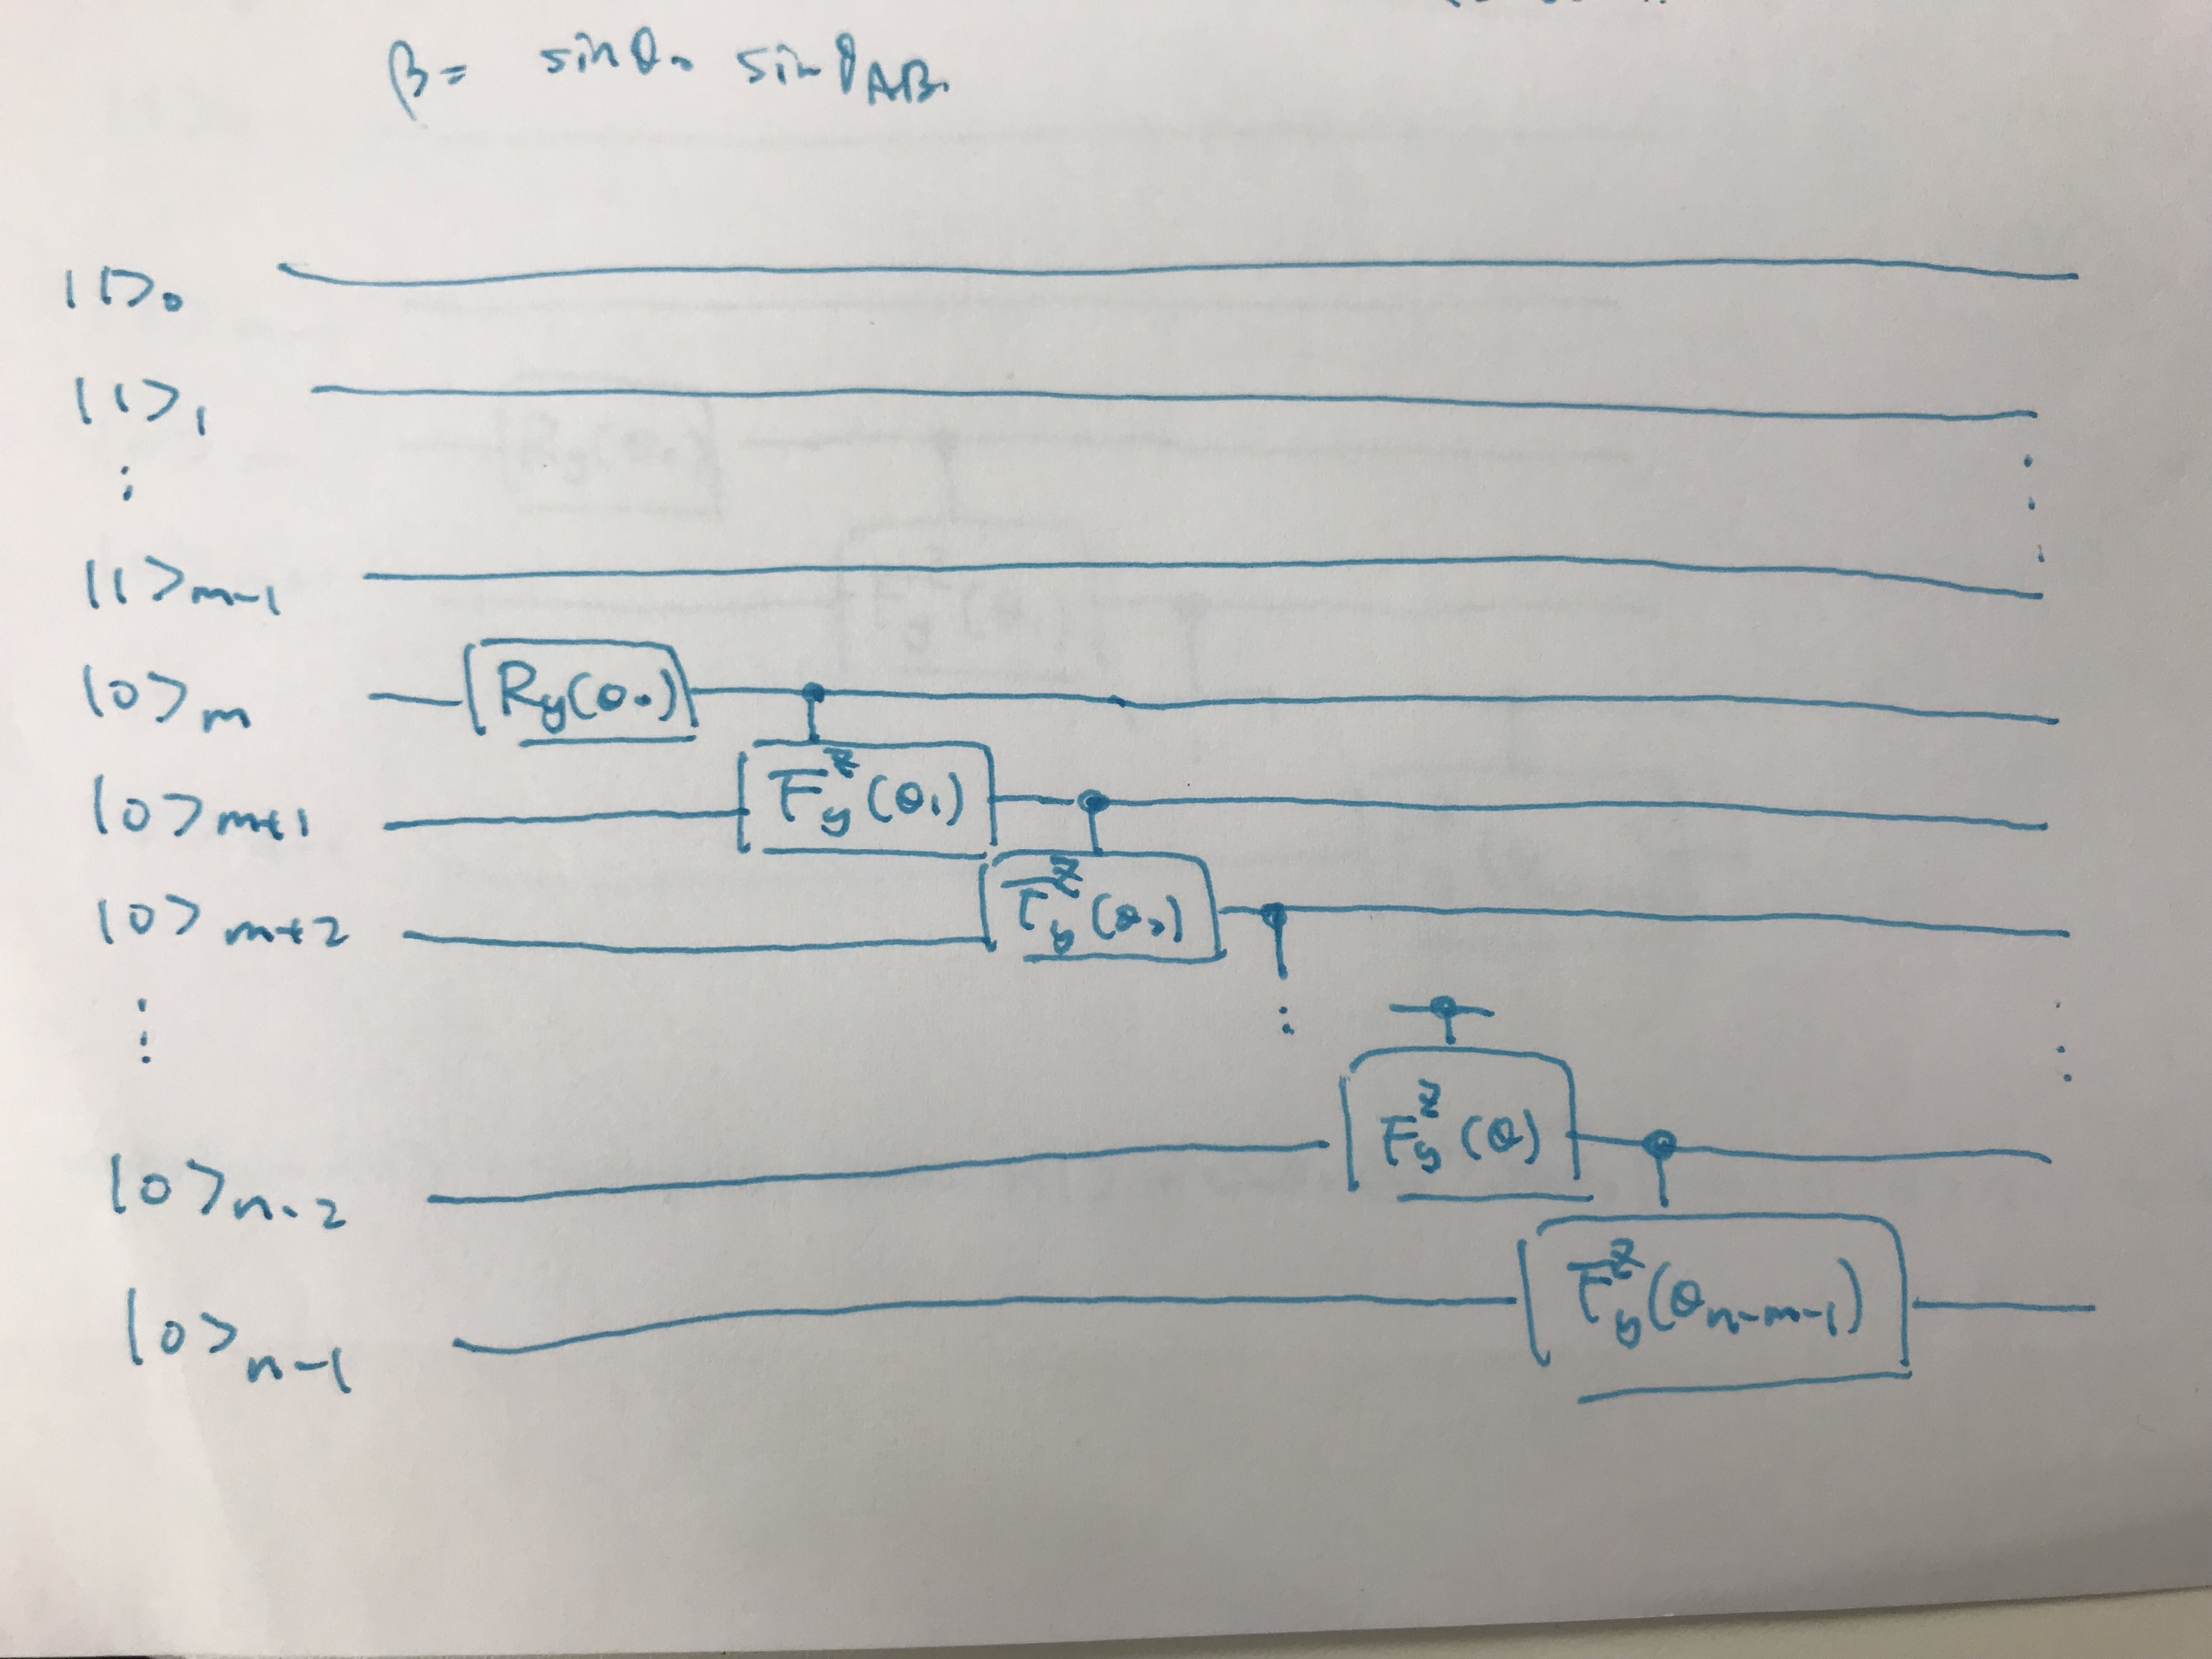
\includegraphics[width=\linewidth]{figs/cis_circuit_01}
\caption{Circuit}
\label{fig:cis}
\end{figure}

Here 
\begin{align}
CF^Z_y(\theta) &= (1 \otimes R_y(\theta)) \mathrm{CZ} (1 \otimes R_y(-\theta)) = 
\begin{bmatrix}
1 & 0 \\
0 & R_y(\theta) Z R_y(-\theta)
\end{bmatrix} \\
R_y(\theta) Z R_y(-\theta) &= 
\begin{bmatrix}
\cos(\theta/2) & -\sin(\theta/2) \\
\sin(\theta/2) & \cos(\theta/2)
\end{bmatrix} 
\begin{bmatrix}
\cos(-\theta/2) & -\sin(-\theta/2) \\
-\sin(-\theta/2) & -\cos(-\theta/2)
\end{bmatrix} \\
&=
\begin{bmatrix}
\cos^2(\theta/2) - \sin^2(\theta/2) & 2 \sin(\theta/2) \cos(\theta/2) \\
2 \sin(\theta/2) \cos(\theta/2) & \sin^2(\theta/2) - \cos^2(\theta/2)
\end{bmatrix} \\
&=
\begin{bmatrix}
\cos(\theta) & \sin(\theta) \\
\sin(\theta) & -\cos(\theta)
\end{bmatrix}
\end{align}

Example: $n=8$, $m=4$. The state we would want to prepare is:
\begin{align}
\ket{\psi} 
=&\cos(\theta_0) \ket{00001111} + \sin(\theta_0) \cos(\theta_1) \ket{00011111} + \sin(\theta_0) \sin(\theta_1) \cos(\theta_2) \ket{00111111}  \\
&+ \sin(\theta_0) \sin(\theta_1) \sin(\theta_2) \cos(\theta_{3}) \ket{01111111} + \sin(\theta_0) \sin(\theta_1) \sin(\theta_2) \sin(\theta_3) \ket{11111111} 
\end{align}

\begin{align}
\ket{00001111} \xRightarrow{R} \cos(\theta_0) \ket{00001111} + \sin(\theta_0) \ket{00011111}
\end{align}

\begin{align}
CF^X_y(\theta) &= (1 \otimes R_y(\theta)) \mathrm{CNOT} (1 \otimes R_y(-\theta)) = 
\begin{bmatrix}
1 & 0 \\
0 & R_y(\theta) X R_y(-\theta)
\end{bmatrix} \\
R_y(\theta) X R_y(-\theta) &= 
\begin{bmatrix}
\cos(\theta/2) & -\sin(\theta/2) \\
\sin(\theta/2) & \cos(-\theta/2)
\end{bmatrix} 
\begin{bmatrix}
\sin(-\theta/2) & \cos(-\theta/2) \\
\cos(-\theta/2) & -\sin(-\theta/2)
\end{bmatrix} \\
&=
\begin{bmatrix}
-2 \sin(\theta/2) \cos(\theta/2) & \cos^2(\theta/2) - \sin^2(\theta/2) \\
- \sin^2(\theta/2) + \cos^2(\theta/2) & 2 \sin(\theta/2) \cos(\theta/2)
\end{bmatrix} \\
&=
\begin{bmatrix}
-\sin(\theta) & \cos(\theta) \\
\cos(\theta) & \sin(\theta)
\end{bmatrix}
\end{align}

\begin{align}
\mathrm{CNOT}_{21} F_y(\theta_{AB}) (R_y(\theta_0) \otimes I) \ket{00} 
= 
\begin{bmatrix}
X & 0 \\
0 & I
\end{bmatrix}
\begin{bmatrix}
1 & 0 \\
0 & R_y(\theta_{AB})
\end{bmatrix}
(\cos(\theta_0) \ket{00} + \sin(\theta_0)\ket{01})
\end{align}

\end{document}  